% SETUP
\documentclass{article}
\usepackage{geometry}
\usepackage{fancyhdr}
\usepackage{titlesec}
\usepackage{tabularx}
\usepackage[none]{hyphenat}
\usepackage{multicol}
\usepackage{hhline}
\usepackage{caption}
\usepackage{graphicx}
\usepackage{biblatex}
\usepackage{amsmath}
\addbibresource{references.bib}
\geometry{
	a4paper, 
	total={170mm,257mm}, 
	left=25mm, 
	right=25mm,
	top=30mm, 
	bottom=30mm}

% FIGURES IN MULTICOLS
\newenvironment{Figure}
  {\par\medskip\noindent\minipage{\linewidth}}
  {\endminipage\par\medskip}

% SECTION TITLE FORMAT
\titleformat{\section}
  {\normalfont\bfseries}{\thesection}{1em}{}[{\titlerule[0.3pt]}]

% HEADER & FOOTER
\pagestyle{fancy}
\renewcommand{\headrulewidth}{0pt}
\chead{\large Progress Report 1 -- Disentanglement by Cross Training \\ \normalfont Naive Approach (7. May 2020)}
\lhead{}
\rhead{}
\cfoot{\thepage}

\begin{document}

% CONTACT
\begin{table}[!h]
\center
\begin{tabular}{|l|l|l|}
\hline
\textbf{Name}             & \textbf{Student ID} & \textbf{E-Mail}            \\ \hhline{|=|=|=|}
Li Nguyen        & 934644485  & li.nguyen@tum.de  \\ \hline
Alexander Koenig & 918254061  & awc.koenig@tum.de \\ \hline
\end{tabular}
\end{table}

% ARCHITECTURES
\begin{figure}[h!]
	\centering 
	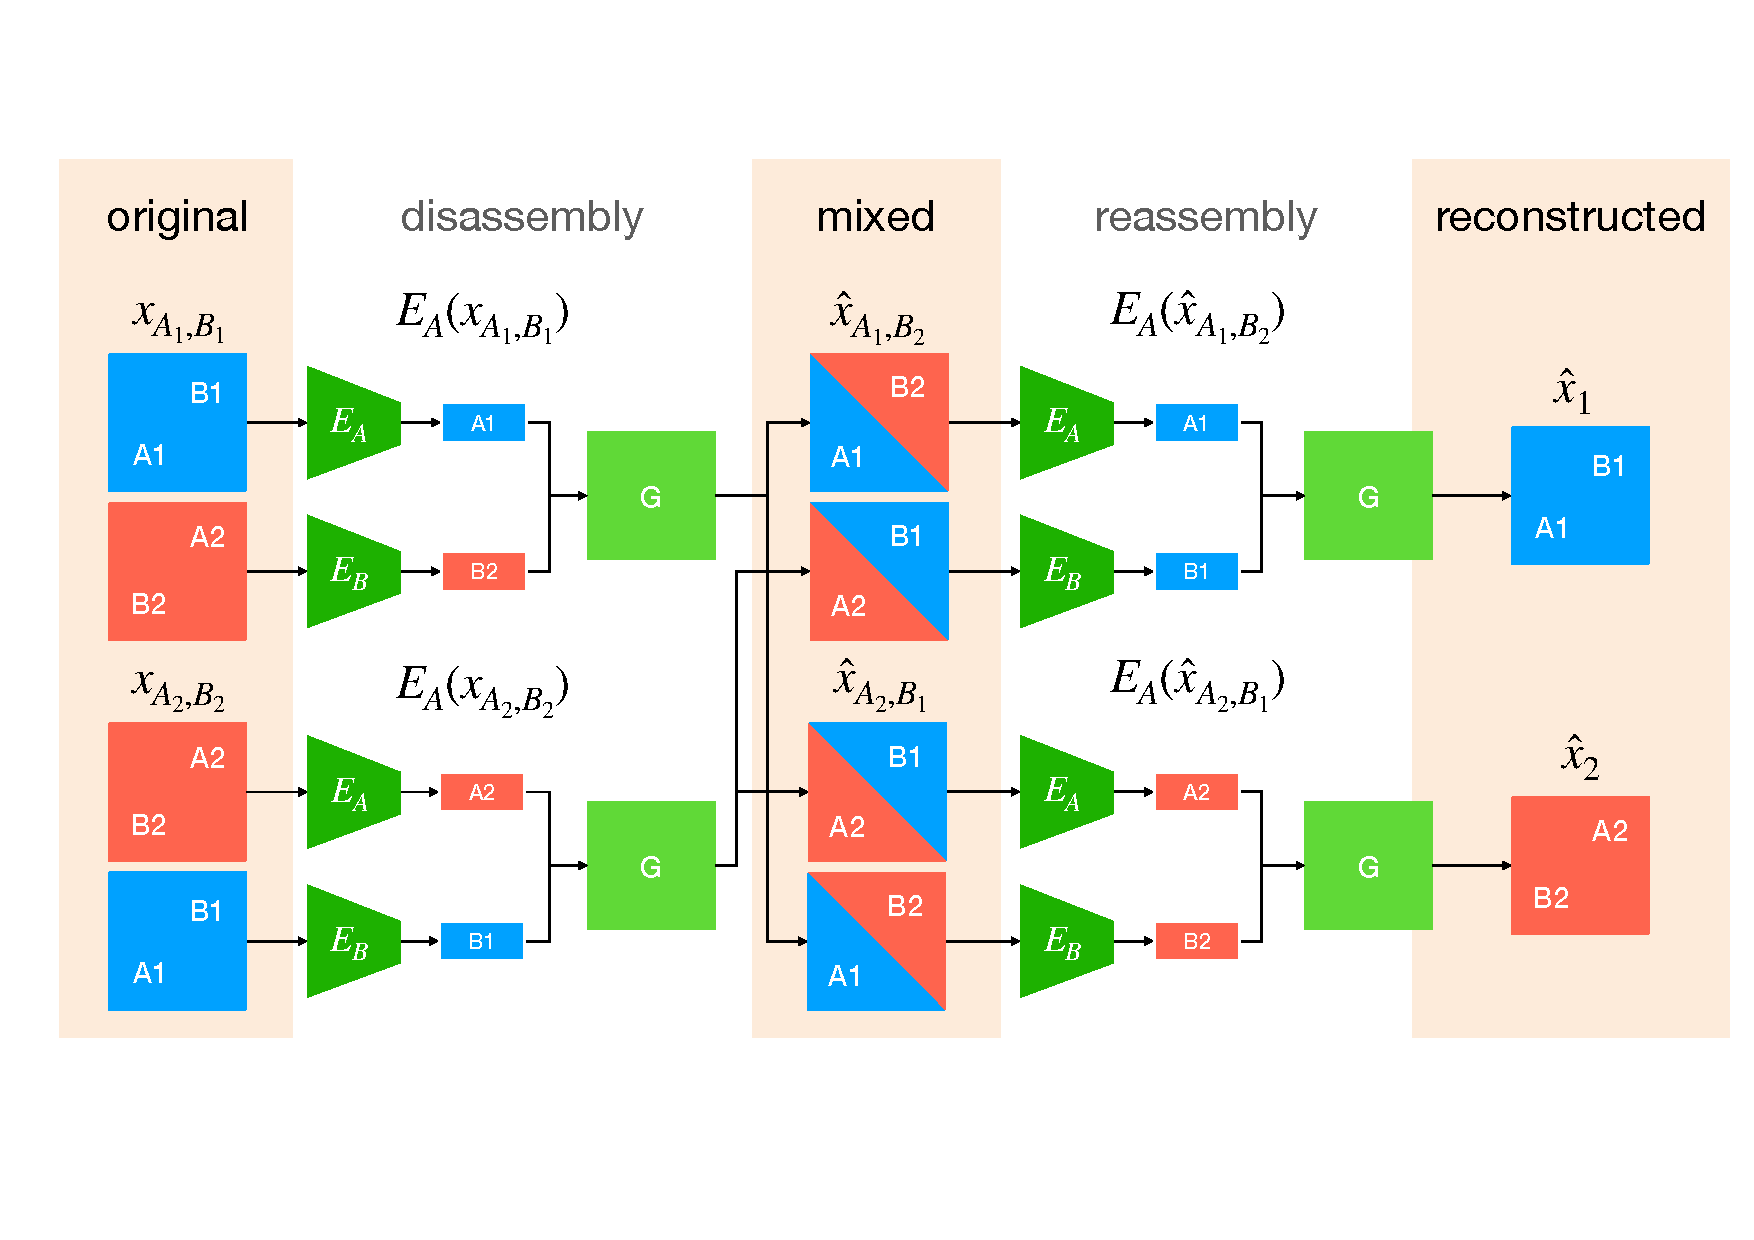
\includegraphics[width=0.9\linewidth]{figures/g2g}
	\caption{Architecture overview}
	\label{fig:g2g}
\end{figure}
\begin{figure}[t]
	\centering 
	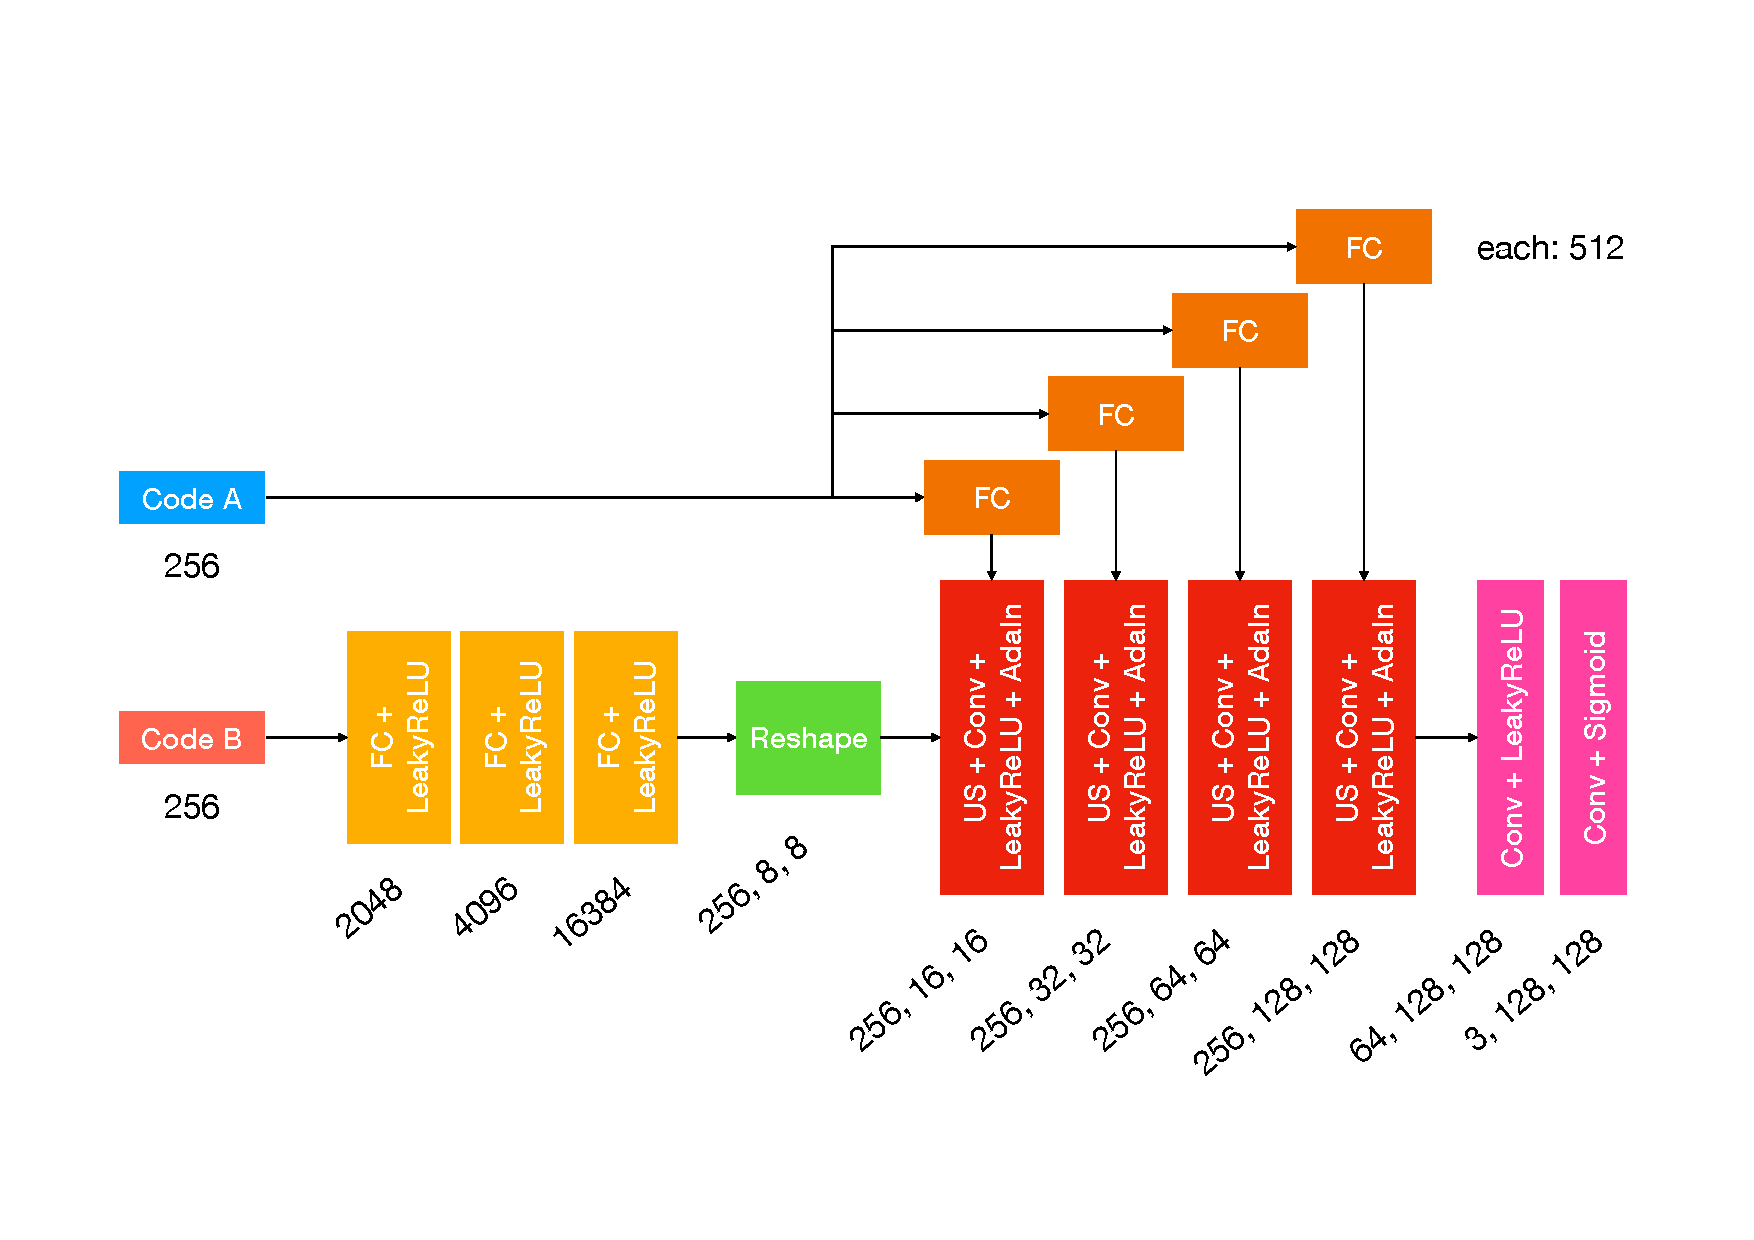
\includegraphics[width=0.9\linewidth]{figures/generator}
	\caption{Generator architecture (\cite{gabbay2020lord} and \cite{LORD})}
	\label{fig:generator}
\end{figure}


\begin{multicols}{2}

\section{Notation}

\begin{itemize}
	\item Original images \\$x_1 = x_{A_1,B_1}$ and $x_2 = x_{A_2,B_2}$
	\item Mixed images \\$\hat{x}_{A_1,B_2} = G \big (E_A(x_1), E_B(x_2) \big)$ and \\$\hat{x}_{A_2,B_1} = G \big (E_A(x_2), E_B(x_1) \big)$
	\item Reconstructed images \\$\hat{x}_1= G \big (E_A(\hat{x}_{A_1,B_2}), E_B(\hat{x}_{A_2,B_1}) \big)  $ and \\$\hat{x}_2  = G \big (E_A(\hat{x}_{A_2,B_1}), E_B(\hat{x}_{A_1,B_2}) \big)  $
\end{itemize}


\section{Architectures}

\textbf{Encoder --} We use the same architecture for both encoder types  (figure \ref{fig:encoders}). The architecture of the encoders is largely based on the paper Mask Based Unsupervised Content Transfer \cite{mokady2019mask}. The encoders consist of 6 [Conv, BatchNorm, LeakyReLU] blocks that convert the input image of size 3*128*128 to a 1D latent code of size 256. 

\textbf{Generator --} The generator was taken from a PyTorch implementation \cite{LORD} of the LORD paper \cite{gabbay2020lord} (figure \ref{fig:generator}). The only modification we did was to use codes of equal size (256). In the original implementation Code A's size was 256 and Code B's size was 128. In the implementation \cite{LORD} Code A is referred to as class code and Code B is called content code. We desire in our implementation that Code A encodes the class (i.e. identity) and Code B encodes the rest of the image. 

The generator first passes Code B through several dense layers with a LeakyReLU activation and then reshapes the output to 256*8*8. Then four [Upsampling, Conv, LeakyReLU, AdaIn] blocks scale the height and width up to the desired 128*128. Each AdaIn normalization layer \cite{huang2017arbitrary} gets two modulation parameters from the dense layers that process the information in the class code A (2 parameters for 256 channels = 512 neurons in FC layers). Finally, two layers and activations aggregate the information into 3 feature maps. 

\begin{Figure}
	\centering 
	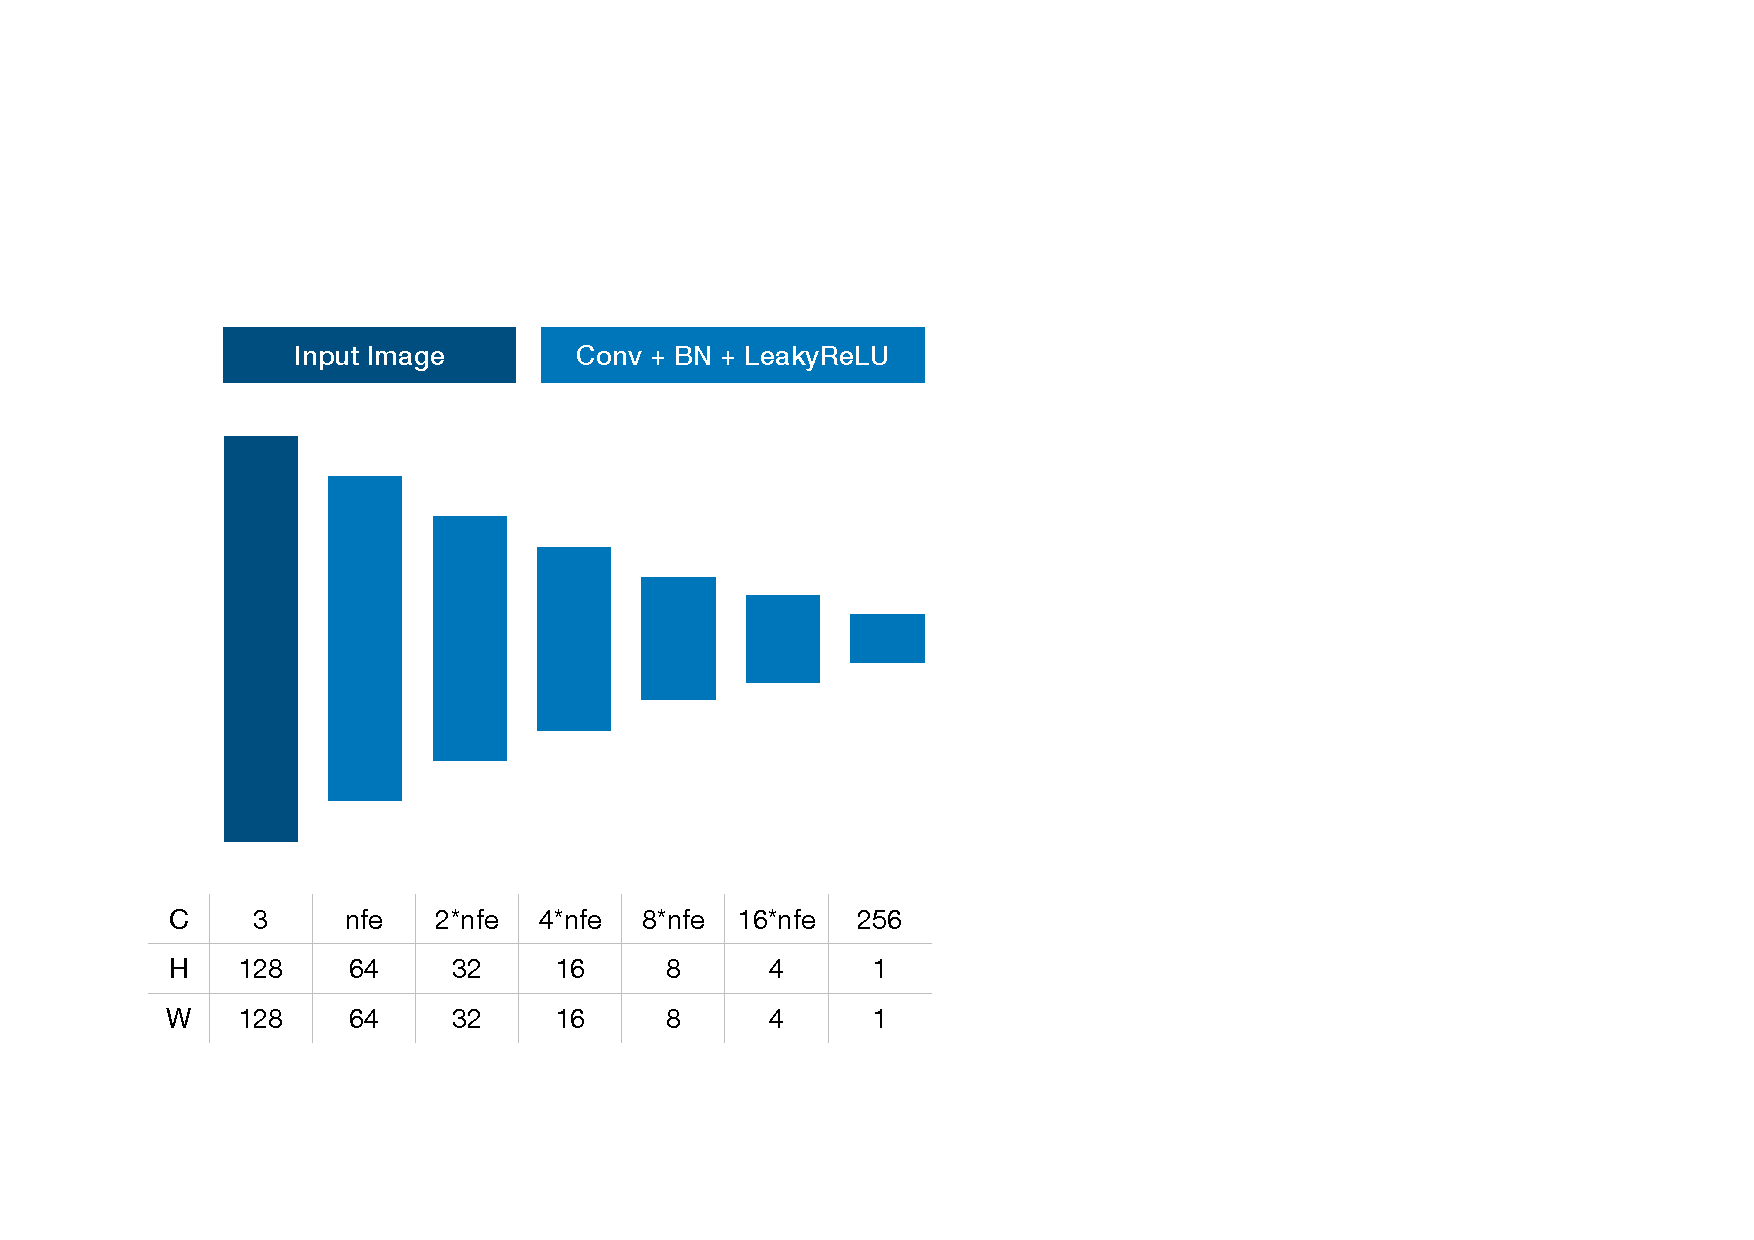
\includegraphics[width=0.75\linewidth]{figures/encoders.pdf}
	\captionof{figure}{Encoder Architecture}
	\label{fig:encoders}
\end{Figure}

\section{Losses}
We use a reconstruction loss for both images in combination with a cycle consistency loss for both encoders. The \textbf{reconstruction loss} is motivated by the fact that the original images should be as similar as possible to the reconstructed images. The \textbf{cycle consistency losses} should guide the network to produce the same low-dimensional embeddings in the disassembly stage as in the reassembly stage (e.g. the feature code $A_1$ should be the same from original image $x_{A_1,B_1}$ as from the mixed image $\hat{x}_{A_1,B_2}$). We define the reconstruction loss in equation \ref{eq:rec} and one cycle consistency loss for each encoder (equations  \ref{eq:cyc1} and \ref{eq:cyc2}).

\begin{equation}
	L_{rec} = \sum_{i=1}^{n} \left\| \hat{x}_i - x_i \right\| 
	\label{eq:rec}
\end{equation}
\begin{multline}
	L_{cyc,E_A} = \sum_{i=1}^{n-1} \left\| E_A(x_{A_i,B_i})- E_A(\hat{x}_{A_i,B_{i+1}})\right\| ^2+ 
	\\
	\left\| E_A(x_{A_{i+1},B_{i+1}}) - E_A(\hat{x}_{A_{i+1},B_i})\right\|^2
	\label{eq:cyc1}
\end{multline}
\begin{multline}
	L_{cyc,E_B} = \sum_{i=1}^{n-1} \left\| E_B(x_{A_i,B_i}) - E_B(\hat{x}_{A_{i+1},B_i})\right\| ^2+ 
	\\
	\left\| E_B(x_{A_{i+1},B_{i+1}}) - E_B(\hat{x}_{A_1,B_{i+1}})\right\|^2
	\label{eq:cyc2}
\end{multline}
\begin{multline}
	L = L_{rec} + \gamma \cdot (L_{cyc,E_A} + L_{cyc,E_B})
	\label{eq:all}
\end{multline}

Finally, we define the overall loss in equation \ref{eq:all}. It is a linear combination of the above losses. We introduce the weighting factor $\gamma$. Both cycle consistency losses are scaled by this parameter. 

As a first milestone we wanted to determine the best performing weight $\gamma$. We trained the model on the CelebA dataset \cite{liu2015faceattributes} with different parameters $\gamma \in [0.01, 0.4, 1, 1.5, 2]$ for 20 epochs with a batch size of 32 (batch size of 64 did not fit on the memory of two GPUs). 

\section{Results}
Figures \ref{fig:train} and \ref{fig:val} show the training and validation losses for all runs. To compare the visual results of the different approaches we introduce a plot with the following layout. 
\begin{Figure}
	\centering 
	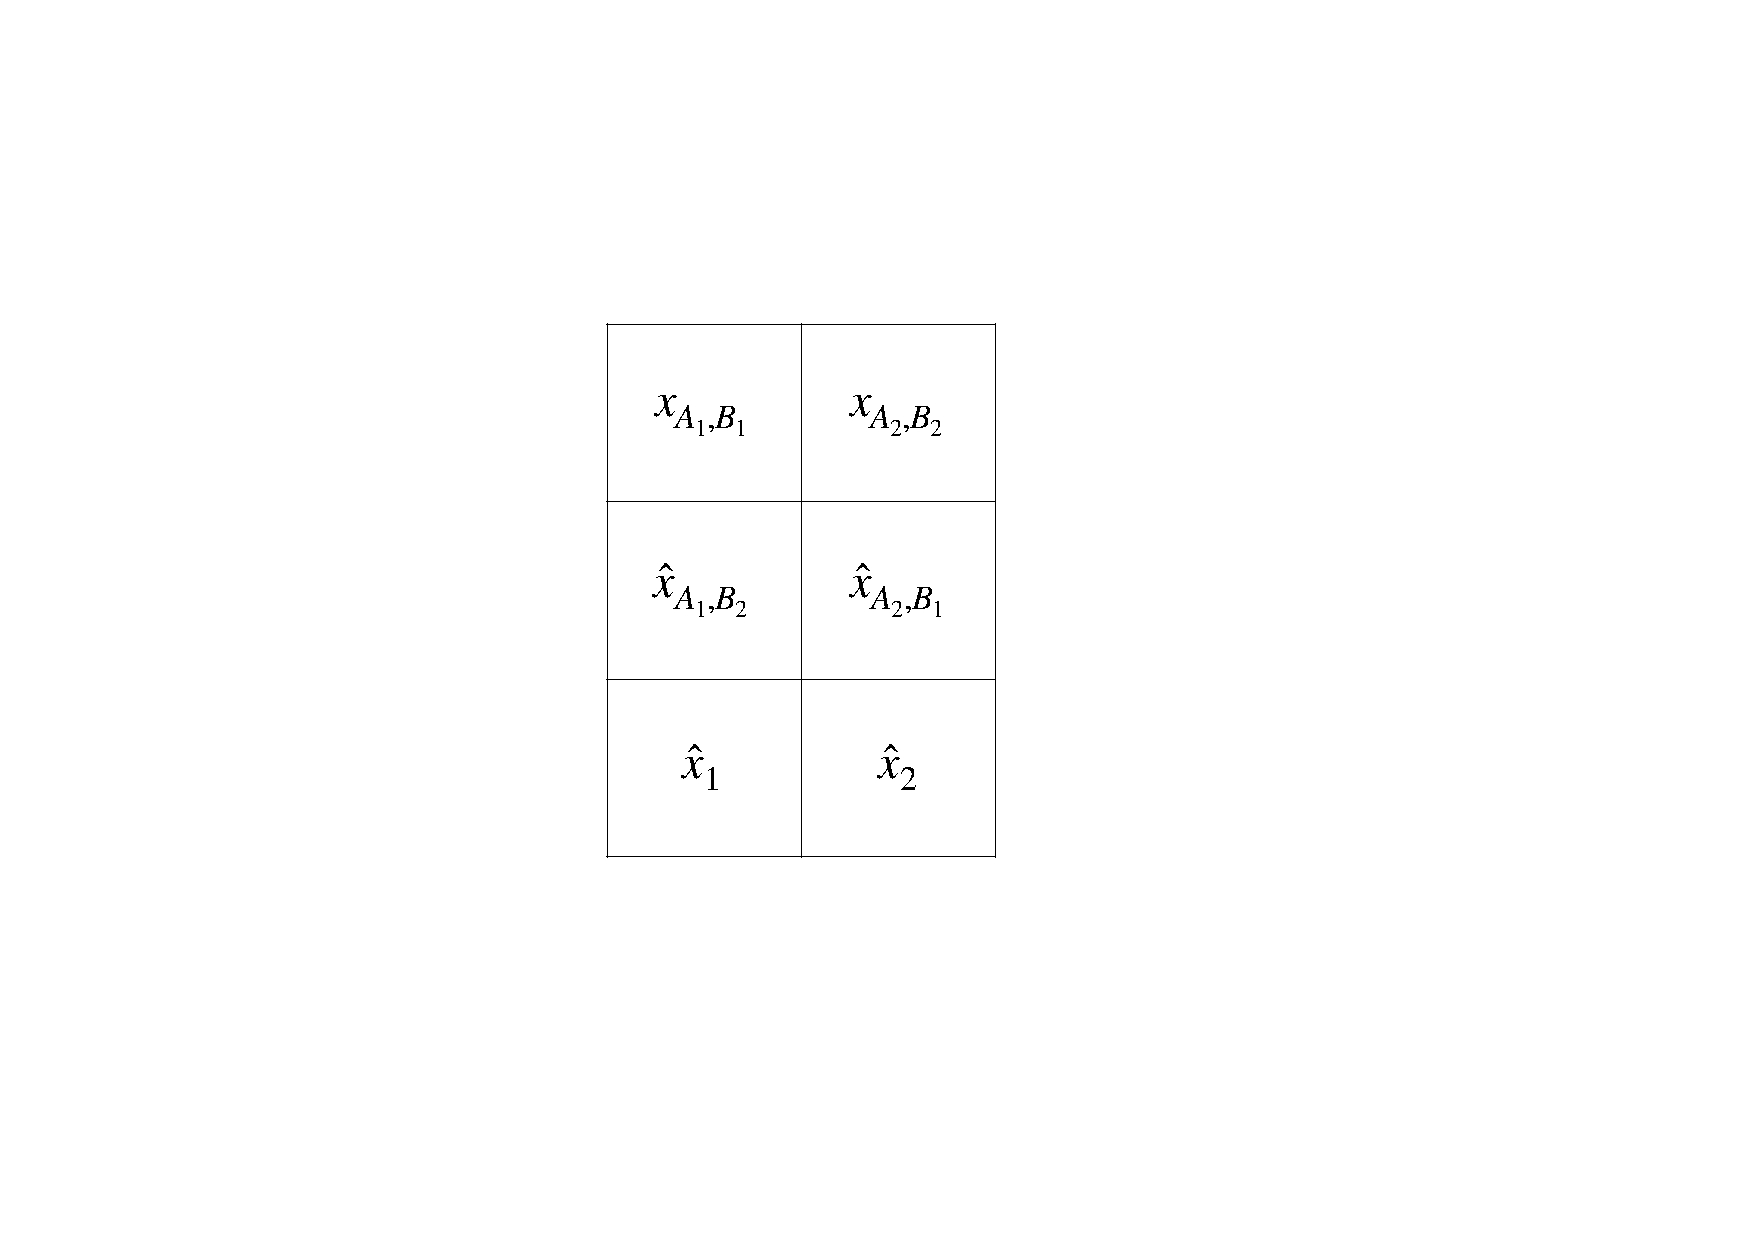
\includegraphics[width=0.5\linewidth]{figures/layout.pdf}
	\captionof{figure}{Layout for plots}
	\label{fig:layout}
\end{Figure}

From the qualitative results in figures \ref{fig:gam_0.01}, \ref{fig:gam_0.4}, \ref{fig:gam_1.0}, \ref{fig:gam_1.5} and \ref{fig:gam_2.0} it becomes clear that a value of $\gamma = 0.4$ performs best. The probably \textbf{best result} can be seen on the far right of figure \ref{fig:gam_0.4} (in red box). The smile from image $x_2$ seems to be successfully transferred to the mixed image $\hat{x}_{A_1,B_2}$. Similarly, the closed mouth of the person in $x_1$ is transferred to the image $\hat{x}_{A_2,B_1}$. Finally, the reconstructed images $\hat{x}_1$ and $\hat{x}_2$ get their original facial expression back. A very small $\gamma$ (0.01) seems to result in a noisy mixed image. For strong $\gamma$ parameters (1.5 and 2.0) the mixed image looks very similar to the reconstructed one. 

\begin{Figure}
	\centering 
	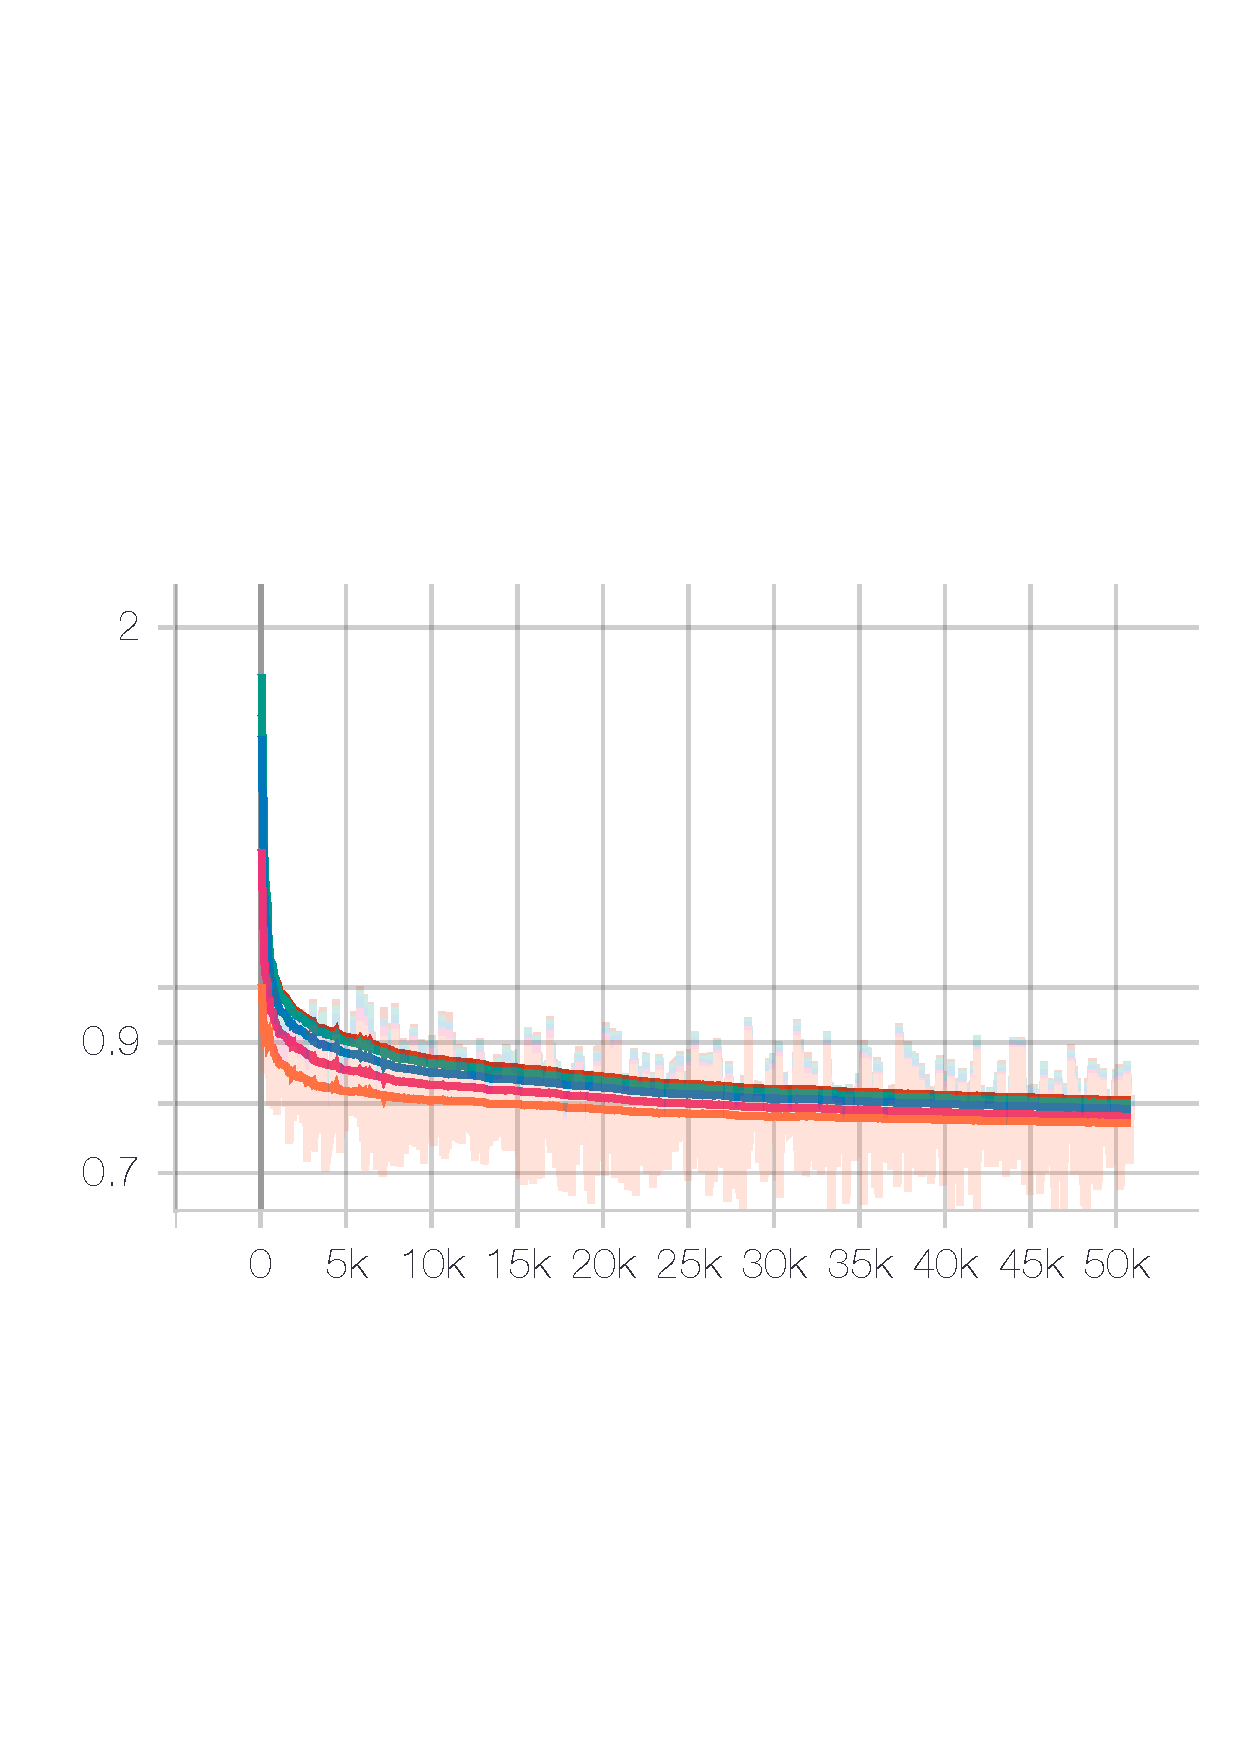
\includegraphics[width=\linewidth]{figures/train_loss}
	\captionof{figure}{Training loss (orange: $\gamma = 0.01$, pink: $\gamma = 0.4$, blue: $\gamma = 1.0$, green:  $\gamma = 1.5$, red = $\gamma = 2.0$)}
	\label{fig:train}
\end{Figure}

\begin{Figure}
	\centering 
	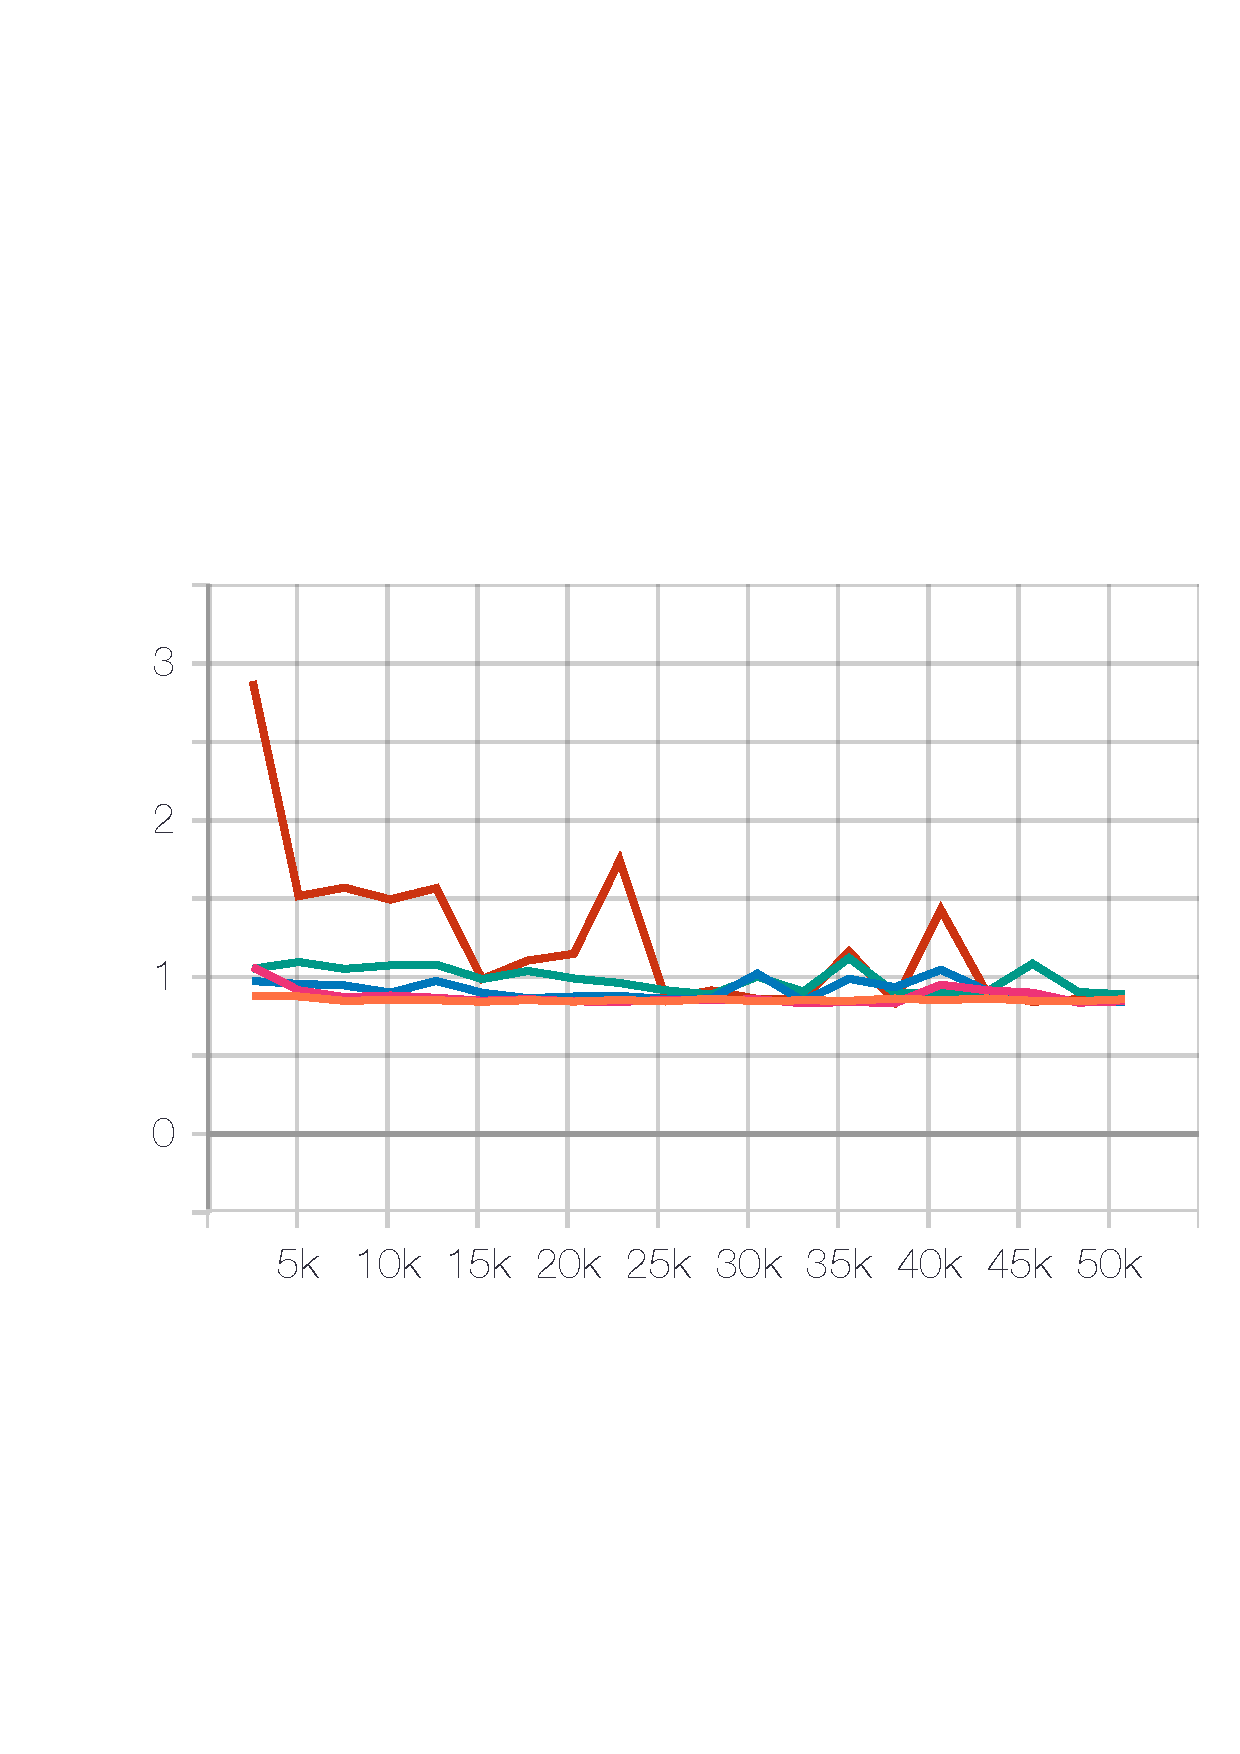
\includegraphics[width=\linewidth]{figures/val_loss}
	\captionof{figure}{Validation loss (orange: $\gamma = 0.01$, pink: $\gamma = 0.4$, blue: $\gamma = 1.0$, green:  $\gamma = 1.5$, red = $\gamma = 2.0$)}
	\label{fig:val}
\end{Figure}

\section{Future Work}
\textbf{Next Steps}
\begin{enumerate}
	\item Run more tests on $\gamma$ values close to 0.4
	\item Implement GAN Loss
\end{enumerate}

\noindent \textbf{Open Questions}
\begin{enumerate}
	\item Should we use a different architecture for $E_A$ than for $E_B$?
	\item Are the sizes of the latent codes suitable? Should the class code $A_i$ be smaller than the code for the rest of the image $B_i$? 
	\item Why are the generated images so pale/grayish?
	\item Is it a good idea to give both cycle consistency losses the same weight (i.e. $\gamma$)?
	\item Does the GAN loss help to generate more detailed images?
	\item Does it make sense to introduce a weight for the GAN loss as well?
	\item Would it improve performance if we increase this weight successively? Specifically, we thought about giving more weight to the discriminator initially to make the discriminator become good in its predictions.
\end{enumerate}
\end{multicols}
\newpage

% RESULTS
\begin{figure}[h!]
	\centering 
	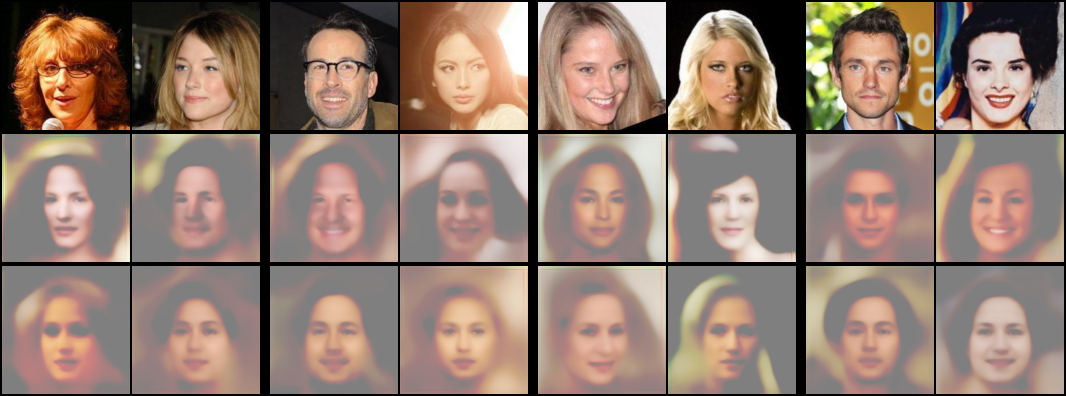
\includegraphics[width=\linewidth]{{figures/gam_0.01}.png}
	\caption{Plots from validation set with $\gamma = 0.01$}
	\label{fig:gam_0.01}
\end{figure}
\begin{figure}[h!]
	\centering 
	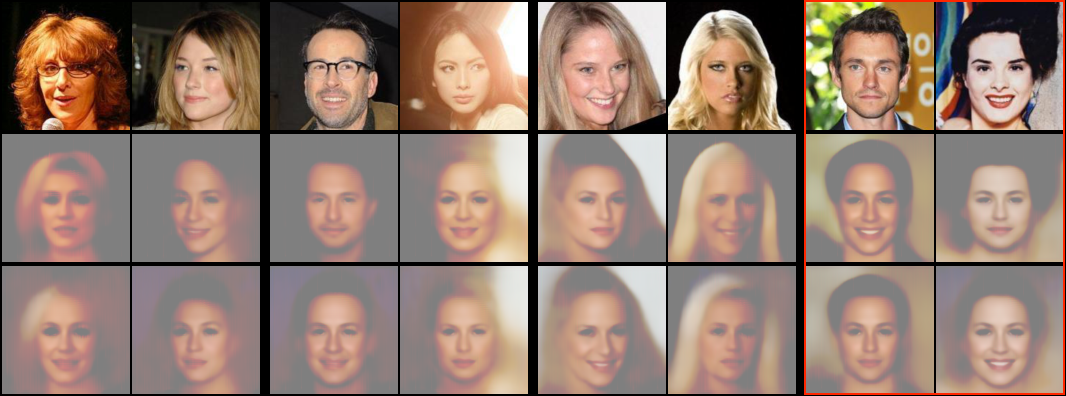
\includegraphics[width=\linewidth]{{figures/gam_0.4}.png}
	\caption{Plots from validation set with $\gamma = 0.4$}
	\label{fig:gam_0.4}
\end{figure}
\begin{figure}[h!]
	\centering 
	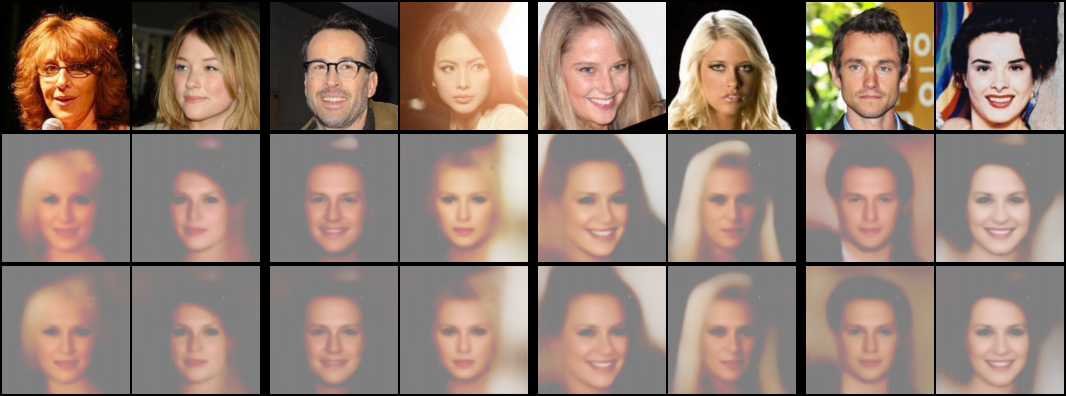
\includegraphics[width=\linewidth]{{figures/gam_1.0}.png}
	\caption{Plots from validation set with $\gamma = 1.0$}
	\label{fig:gam_1.0}
\end{figure}
\begin{figure}[h!]
	\centering 
	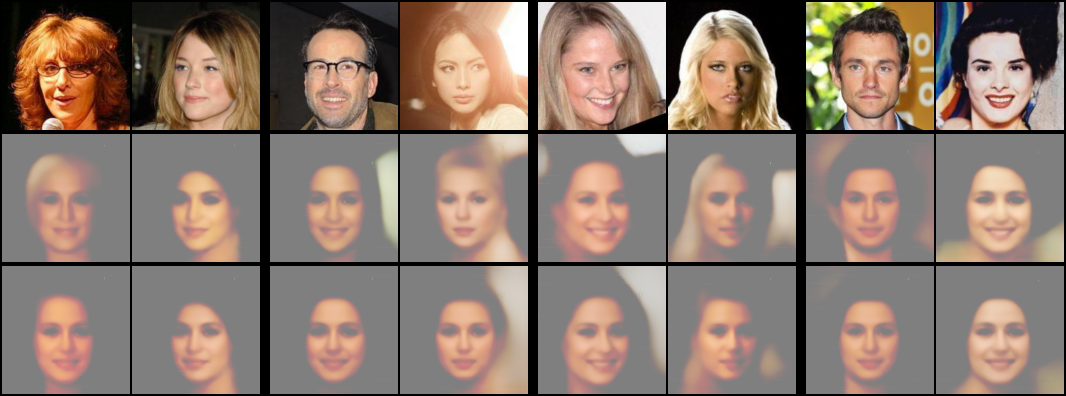
\includegraphics[width=\linewidth]{{figures/gam_1.5}.png}
	\caption{Plots from validation set with $\gamma = 1.5$}
	\label{fig:gam_1.5}
\end{figure}
\begin{figure}[h!]
	\centering 
	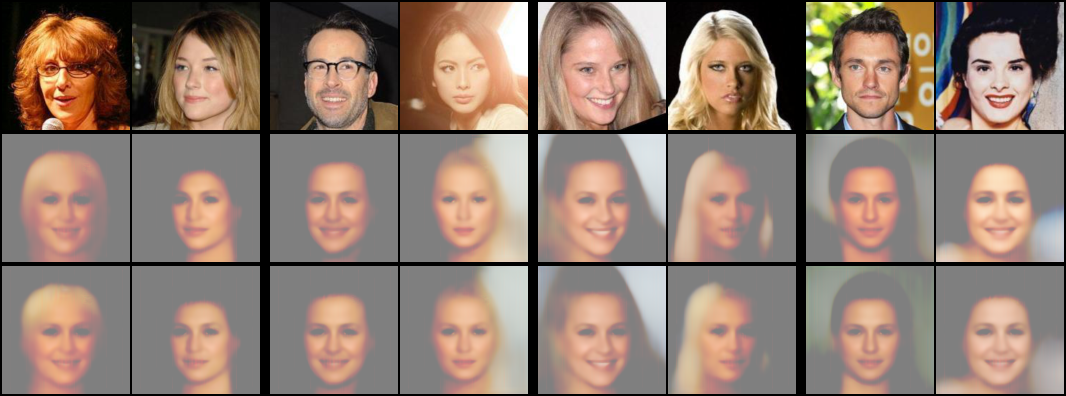
\includegraphics[width=\linewidth]{{figures/gam_2.0}.png}
	\caption{Plots from validation set with $\gamma = 2.0$}
	\label{fig:gam_2.0}
\end{figure}

\printbibliography

\end{document}